Um das Phänomen der Influenz und vieles Weitere rund um die Elektrizität zu beschreiben, wurde das Modell des elektrischen Feldes entwickelt. 

\begin{NiceToKnow}
Generell geht es in der Physik nicht unbedingt darum, zu erläutern, wie etwas genau funktioniert, da vieles, wie zum Beispiel die eigentliche Beschaffenheit von Feldern, (noch) gar nicht genau zu erklären ist. Es geht darum, Modelle zu entwickeln, mit deren Hilfe sich mathematische Ausdrücke zur Beschreibung von diesen Phänomenen ableiten lassen.
\end{NiceToKnow}


\subsection{Feldlinien}

\begin{figure}[h!]
	\centering
	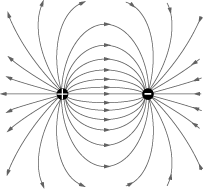
\includegraphics[width=0.9\textwidth]{EFeld}
	\caption{Feldlinien zwischen zwei geladenen Teilchen}
\end{figure}

Feldlinien\endnote{\glqq Camposcargas\grqq{} by http://commons.wikimedia.org/wiki/User:Chanchocan - Own work. Licensed under CC BY-SA 3.0 via Commons - \url{https://commons.wikimedia.org/wiki/File:Camposcargas.PNG}} sind ein Modell zur Verdeutlichung von grundlegenden Eigenschaften eines elektrischen Feldes. Sie schneiden sich nie und haben eine Richtung, die durch Pfeile angezeigt wird. Sollten sie von einem Körper ausgehen oder auf einen Körper auftreffen, stehen sie senkrecht auf dessen Oberfläche. Außerdem gibt die Dichte der Linien die Stärke des Feldes an.\endnote{Paragraph von: Armin Kunz: \glqq Bewertung der 1. Klausur\grqq{} vom 09.10.2014} Die Pfeile der Feldlinien zeigen immer zum negativen Pol.

Bei der Wechselwirkung zweier Körper gibt es eine abstoßende Kraftwirkung bei gegenläufigen Feldlinien und eine anziehende Kraftwirkung, wenn die Feldlinien in dieselbe Richtung zeigen.


\subsection{Coulomb'sches Gesetz} \label{subsec:CoulombGesetz}

Wenn nun klar ist, dass sich Ladungen beeinflussen, ist der nächste Schritt diesen \glqq Einfluss\grqq{} mathematisch auszudrücken. Dazu gibt es das Coulomb'sche Gesetz, welches die Kraft, die zwei kugelförmige (sphärische) Körper aufeinander auswirken, in Abhängigkeit von deren Ladungen und dem Abstand, angibt:

\begin{equation} \label{eq:coulomb_gesetz}
	F = \frac{1}{4\pi \cdot \epsilon_0} \cdot \frac{Q_1 \cdot Q_2}{d^{2}}
\end{equation}

Die Gleichung besteht aus einem konstanten Faktor, der die sogenannte \glqq Permittivität\grqq{} (\glqq elektrische Feldkonstante\grqq ) $\epsilon_0$ beinhaltet (\casio{32}), und einem variablen Teil der die Beträge der beiden Ladungen $Q_1$ und $Q_2$, und den Abstand der Mittelpunkte $d$ enthält.

Die Einheit Ladung ist $C$ (sprich: \glqq Coulomb\grqq ), was gleich $A \cdot s$ ist. Dies folgt daraus, dass Stromstärke als Ladung pro Zeit ($\frac{Q}{t}$) definiert ist; daher kann man Ladung als Stromstärke \emph{mal} Zeit ($A \cdot t$).

Eine Einheitenrechnung sieht dann wie folgt aus:

\begin{align}\label{eq:coulomb_gesetz_einheiten}
\begin{split}
	N 							&= \frac{1}{\epsilon_0} \cdot \frac{As \cdot As}{m^{2}} \\
	\frac{kg \cdot m}{s^{2}} 	&= \frac{1}{\epsilon_0} \cdot \frac{A^{2} \cdot s^{2}}{m^{2}}
\end{split}
\end{align}

\noindent Daraus ergibt sich als Einheit für die Feldkonstante $\epsilon_0$:

\begin{align}\label{eq:feldkonstante_einheiten}
\begin{split}
	\epsilon_0 &= \frac{A^{2} \cdot s^{2}}{m^{2}} \cdot \frac{s^{2}}{kg \cdot m} \\
	\epsilon_0 &= \frac{A^{2} \cdot s^{4}}{m^{3} \cdot kg} \\
	\epsilon_0 &= \frac{As}{Vm}
\end{split}
\end{align}

\begin{Aufgabe}
Versuche über die Definition des Volts ($V=\frac{kg \cdot m^2}{A \cdot s^3}$) von der vorletzten auf die letzte Umformung zu kommen! Einheitenrechnungen sind wichtig!
\end{Aufgabe}

\begin{NiceToKnow}
Diese Form der Gleichung ist analog zu Newtons Gravitationsgesetz: $F = G \cdot \frac{m_1 \cdot m_2}{d^2}$. Hierbei ist $G$ ebenfalls eine Konstante, nämlich die Gravitätskonstante.
\end{NiceToKnow}


\subsection{Homogenes Feld} \label{subsec:EFeldHomogen}

Das elektrische Feld zwischen zwei geladenen Körpern ist meistens inhomogen. Das heißt, dass die Feldstärke, also die Dichte der Feldlinien nicht überall gleich ist. Für Berechnungen würde dies das Lösen von komplexen Differentialgleichungen voraussetzen. Daher wird in der Schulphysik fast immer von einem homogenen Feld ausgegangen, wenn Berechnungen an einem elektrischen Feld anstehen:

\begin{itemize}
	\item Die Feldlinien sind alle parallel.
	\item Die Feldlinien zeigen alle in dieselbe Richtung.
	\item Die Feldlinien haben alle denselben Abstand zueinander.
\end{itemize} 

\noindent Eine Möglichkeit, so ein Feld zu generieren, ist der Plattenkondensator (\referenz{sec:plattenkondensator}).


\subsection{Feldstärke}  \label{subsec:Feldstaerke}

In einem homogenen Feld ist die Feldstärke (Formelzeichen: $E$) also an jedem Punkt gleich. Sie ordnet jedem geladenen Körper eine Kraft und, würde man mit Vektoren rechnen, eine Richtung zu:

\begin{equation} \label{eq:feldstaerke}
	\vec{E} = \frac{\vec{F}}{q}
\end{equation}

\noindent $q$ ist hierbei die \emph{vorzeichenbehaftete} Ladung des Probekörpers im Feld. Als Einheit ergibt sich $\frac{N}{C}$ für die Feldstärke $E$. 

Umgeformt für $F$ ergibt sich aus der Gleichung:

\begin{equation} \label{eq:feldstaerke_nach_F}
	\vec{F} = q \cdot \vec{E}
\end{equation}








